\documentclass[10pt]{article}
\usepackage[utf8]{inputenc}
\usepackage{pgfplots}
\pgfplotsset{compat=1.15}
\usepackage{mathrsfs}
\usetikzlibrary{arrows}
\pagestyle{empty}
\begin{document}
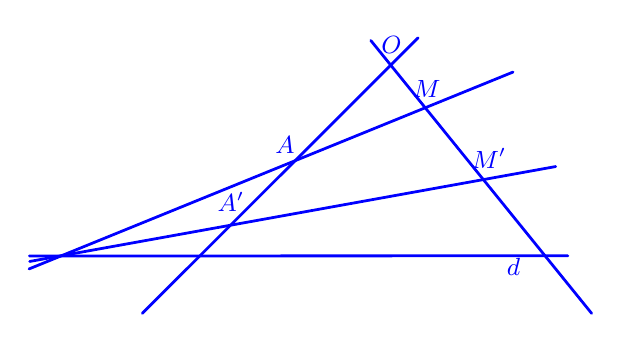
\begin{tikzpicture}[scale=1.3,line cap=round,line join=round,>=latex,x=1.0cm,y=1.0cm]
%\begin{axis}[x=1.0cm,y=1.0cm, axis lines=middle, ymajorgrids=true,xmajorgrids=true,xmin=0,
xmax=5.6,ymin=0,ymax=2.8,
xtick={0,1,...,5},
ytick={0,1,...,2.8}]
%\clip(-2.9053341830801167,-2.6854622518378726) rectangle (7.610615397688167,4.445215888546074);
\draw [line width=1.pt,color=blue] (1.1104573698878413,0.)-- (3.804529959989662,2.691578176978554);
\draw [line width=1.pt,color=blue] (3.3426889445436356,2.665920342787108)-- (5.5,0.);
\draw [line width=1.pt,color=blue] (0.010255800991182958,0.5070288028442502)-- (5.149000471621427,1.4343443015977126);
\draw [line width=1.pt,color=blue] (0.004217693802966688,0.4340855753598525)-- (4.732184842681713,2.357345348309727);
\draw [line width=1.pt,color=blue] (0.0077948153920701846,0.5611704860247311)-- (5.268223314572802,0.5619951529263205);
\begin{small}
%\draw [fill=blue] (1.9812329497927719,0.869969338067975) circle (2.5pt);
\draw[color=blue] (1.976499336150213,1.0879549683540815) node {$A'$};
%\draw [fill=blue] (2.603113201401751,1.4912737973740986) circle (2.0pt);
\draw[color=blue] (2.504697716919396,1.6401623664309528) node {$A$};
%\draw [fill=blue] (3.537672284879562,2.424967582548197) circle (2.0pt);
\draw[color=blue] (3.5450884669193026,2.624532076046245) node {$O$};
%\draw [fill=blue] (3.8746679954520276,2.0085215081748014) circle (2.0pt);
\draw[color=blue] (3.8892177149961946,2.192369764507824) node {$M$};
%\draw [fill=blue] (4.442475073838538,1.3068478032074407) circle (2.0pt);
\draw[color=blue] (4.497446153457678,1.5121142741232725) node {$M'$};
%\draw [fill=blue] (4.7151903264812045,0.4210381770468915) circle (2.5pt);
\draw[color=blue] (4.737536326534579,0.45571751258491) node {$d$};
\end{small}
%\end{axis}
\end{tikzpicture}
\end{document} 